

\tikzset{every picture/.style={line width=0.75pt}} %set default line width to 0.75pt        

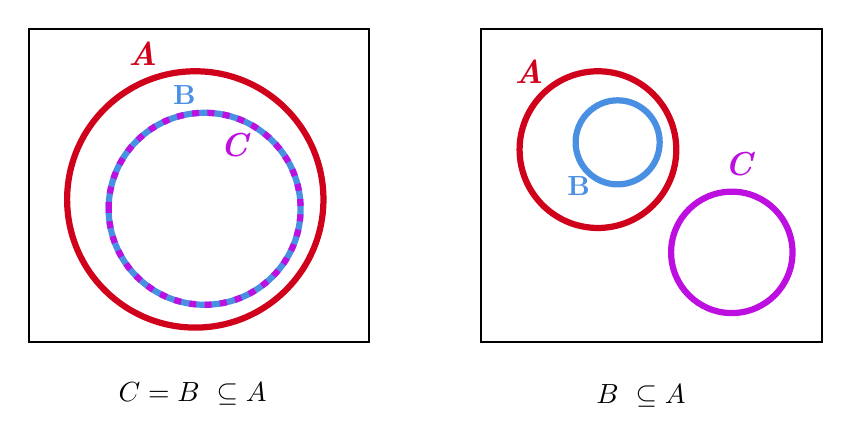
\begin{tikzpicture}[x=0.75pt,y=0.75pt,yscale=-1,xscale=1]
%uncomment if require: \path (0,214); %set diagram left start at 0, and has height of 214

%Shape: Circle [id:dp4028878273251244] 
\draw  [color={rgb, 255:red, 208; green, 2; blue, 27 }  ,draw opacity=1 ][line width=2.25]  (378.5,75.25) .. controls (378.5,54.4) and (395.4,37.5) .. (416.25,37.5) .. controls (437.1,37.5) and (454,54.4) .. (454,75.25) .. controls (454,96.1) and (437.1,113) .. (416.25,113) .. controls (395.4,113) and (378.5,96.1) .. (378.5,75.25) -- cycle ;
%Shape: Circle [id:dp4248744845188792] 
\draw  [color={rgb, 255:red, 74; green, 144; blue, 226 }  ,draw opacity=1 ][line width=2.25]  (405.5,71.75) .. controls (405.5,60.57) and (414.57,51.5) .. (425.75,51.5) .. controls (436.93,51.5) and (446,60.57) .. (446,71.75) .. controls (446,82.93) and (436.93,92) .. (425.75,92) .. controls (414.57,92) and (405.5,82.93) .. (405.5,71.75) -- cycle ;
%Shape: Circle [id:dp42245798174016436] 
\draw  [color={rgb, 255:red, 189; green, 16; blue, 224 }  ,draw opacity=1 ][line width=2.25]  (451.5,124.75) .. controls (451.5,108.6) and (464.6,95.5) .. (480.75,95.5) .. controls (496.9,95.5) and (510,108.6) .. (510,124.75) .. controls (510,140.9) and (496.9,154) .. (480.75,154) .. controls (464.6,154) and (451.5,140.9) .. (451.5,124.75) -- cycle ;
%Shape: Rectangle [id:dp15291346971923803] 
\draw   (360,17) -- (524,17) -- (524,168) -- (360,168) -- cycle ;
%Shape: Circle [id:dp29321322791155224] 
\draw  [color={rgb, 255:red, 208; green, 2; blue, 27 }  ,draw opacity=1 ][line width=2.25]  (160.5,99.25) .. controls (160.5,65.15) and (188.15,37.5) .. (222.25,37.5) .. controls (256.35,37.5) and (284,65.15) .. (284,99.25) .. controls (284,133.35) and (256.35,161) .. (222.25,161) .. controls (188.15,161) and (160.5,133.35) .. (160.5,99.25) -- cycle ;
%Shape: Circle [id:dp04485918012514878] 
\draw  [color={rgb, 255:red, 74; green, 144; blue, 226 }  ,draw opacity=1 ][line width=2.25]  (180.5,103.75) .. controls (180.5,78.21) and (201.21,57.5) .. (226.75,57.5) .. controls (252.29,57.5) and (273,78.21) .. (273,103.75) .. controls (273,129.29) and (252.29,150) .. (226.75,150) .. controls (201.21,150) and (180.5,129.29) .. (180.5,103.75) -- cycle ;
%Shape: Circle [id:dp59798250789504] 
\draw  [color={rgb, 255:red, 189; green, 16; blue, 224 }  ,draw opacity=1 ][dash pattern={on 2.53pt off 3.02pt}][line width=2.25]  (180.5,103.75) .. controls (180.5,78.21) and (201.21,57.5) .. (226.75,57.5) .. controls (252.29,57.5) and (273,78.21) .. (273,103.75) .. controls (273,129.29) and (252.29,150) .. (226.75,150) .. controls (201.21,150) and (180.5,129.29) .. (180.5,103.75) -- cycle ;
%Shape: Rectangle [id:dp1165455056964333] 
\draw   (142,17) -- (306,17) -- (306,168) -- (142,168) -- cycle ;

% Text Node
\draw (484,82) node [scale=1,color={rgb, 255:red, 80; green, 227; blue, 194 }  ,opacity=1 ] [align=left] {{\large \textbf{\textit{\textcolor[rgb]{0.74,0.06,0.88}{C}}}}};
% Text Node
\draw (407,93) node [scale=1,color={rgb, 255:red, 80; green, 227; blue, 194 }  ,opacity=1 ] [align=left] {\textcolor[rgb]{0.29,0.56,0.89}{\textbf{B}}};
% Text Node
\draw (383,38) node [scale=1,color={rgb, 255:red, 245; green, 166; blue, 35 }  ,opacity=1 ] [align=left] {\textit{\textcolor[rgb]{0.82,0.01,0.11}{{\large \textbf{A}}}}};
% Text Node
\draw (437,194) node   {$B\ \subseteq A$};
% Text Node
\draw (197,29) node [scale=1,color={rgb, 255:red, 245; green, 166; blue, 35 }  ,opacity=1 ] [align=left] {\textit{\textcolor[rgb]{0.82,0.01,0.11}{{\large \textbf{A}}}}};
% Text Node
\draw (217,49) node [scale=1,color={rgb, 255:red, 80; green, 227; blue, 194 }  ,opacity=1 ] [align=left] {\textcolor[rgb]{0.29,0.56,0.89}{\textbf{B}}};
% Text Node
\draw (241,73) node [scale=1,color={rgb, 255:red, 80; green, 227; blue, 194 }  ,opacity=1 ] [align=left] {{\large \textbf{\textit{\textcolor[rgb]{0.74,0.06,0.88}{C}}}}};
% Text Node
\draw (221,193) node   {$C=B\ \subseteq A$};


\end{tikzpicture}